\section{Modelling the Trajectory travelled by each robot}

We know that the length of the trajectory travelled by the robot can be represented by the following integral:

\begin{align*}
    L_j &= \int_{0}^{1}|P_j'(t)| \ dt \text{ for } j = 1,...,N \\
        &= \int_{0}^{1} \sqrt{\bigg(\frac{dx_j}{dt}\bigg)^2 + \bigg(\frac{dy_j}{dt}\bigg)^2}.
\end{align*}

We can use the equation above to find the total length of the trajectories travelled by \( N \) robots. Hence, we have that    %Should I mention velocity here or in the objective? I added it at the end 
\begin{align*}
    L(P_1,..,P_N) &= \sum_{j=1}^{N}L_j 
                  = \sum_{j=1}^{N} \bigg[\int_{0}^{1} |P_j'(t)| \ dt \bigg] \\ 
   \implies L(P_1,..,P_N) &= \int_{0}^{1} \bigg[ \sum_{j=1}^{N} |P_j'(t)|\bigg] \ dt. 
\end{align*}
Hence,
\begin{align*}
    L(P_1,..,P_N) &= \int_{0}^{1}|P'(t)| \ dt. \\
    \text{where } |P'(t)| &= \sum_{j=1}^{N}\bigg| \frac{dP_j}{dt}\bigg| \\
                          &= \sum_{j=1}^{N} \sqrt{\bigg(\frac{dx_j}{dt}\bigg)^2 + \bigg(\frac{dy_j}{dt}\bigg)^2}.
\end{align*}

Minimizing this functional will create the shortest trajectory for each robot. Given that the robots must travel the distance within the time period [0,1], it follows that the shortest trajectories will also result in the smallest required velocities. This is because the longer the path, the faster the robot must move to get from start point to end point in the set time. 


\section{Modelling Repulsion Between Robots}

In this section, we will use Coulomb's law to model our situation.

\subsection{Background on Coulomb's Law}

\begin{itemize}
    \item Let \( q_1 \) and \( q_2 \) be two charges. They experience an electrostatic force of attraction or repulsion.
\begin{center}
\begin{tikzpicture}

\draw[->](-1,0)  -- (-3,0);;

\draw[->](1,0) -- (3,0);;

\node[circle,inner sep=1pt,fill=black,label=left:{$-q_2$}] at (1,0) {};

\node[circle,inner sep=1pt,fill=black,label=right:{$-q_1$}] at (-1,0) {};


\end{tikzpicture}  
    
\end{center}

\begin{center}
\begin{tikzpicture}

\draw[->](-3,0) -- (-1,0);

\draw[->](3,0) -- (1,0);

\node[circle,inner sep=1pt,fill=black,label=right:{$ +q_2$}] at (3,0) {};

\node[circle,inner sep=1pt,fill=black,label=left:{$-q_1$}] at (-3,0) {};

\end{tikzpicture}  
    
\end{center}
 \item The magnitude of the electrostatic force is inversely proportional to the square of the distance between them:
    \begin{align*}
        |F| = K\frac{|q_1||q_2|}{r^2}
    \end{align*}
    where \( |F| \) represents the magnitude of force, \( K \) is Coulomb's constant, \( q_1,q_2 \)  are the particle charges, and \( r \) is the distance between \( q_1 \) and \( q_2 \).  
\end{itemize}

Note that the closer the two particles are, the larger the force. We incorporate this idea into our situation by viewing each robot as a moving particle with charge \( q_j \). We want to minimize the force between them which results in maximizing the distance between them, therefore preventing collision.

Our assumption is that all the robots are identical. Therefore, they have the same charge \( q \). Hence, at a fixed time \( t \), the magnitude of the force \( F_j \) between each robot \( i \) and \(j \) is:

\begin{align*}
    |F_{ij}| = K\frac{Q^2}{|P_i(t) - P_j(t)|^2}.
\end{align*}

But, we need to evaluate the force \( F_{ij} \) over continuous time. 

We consider the following equal subdivision of the travel time interval \( [0,1] \):

\begin{center}
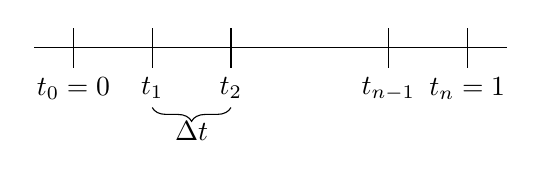
\begin{tikzpicture}
\foreach \x/\y in {0/t_0 = 0, 1/t_1, 2/t_2 , 4/t_{n-1}, 5/t_n = 1 }
 \draw (\x,0.25) -- (\x,-0.25) node[below]{$\y$};
\draw(-0.5,0)--(5.5,0);
\draw [decorate,decoration={brace,amplitude=5pt,mirror,raise=5ex}]
  (1,0) -- (2,0) node[midway,yshift=-3em]{$\Delta t$};
\end{tikzpicture}
\end{center}


where we have \( n \) subintervals \( [t_{\ell}, t_{\ell + 1}] \) and \( \Delta t = \frac{1-0}{n} = \frac{1}{n} \). We assume that every time step \( \Delta t \) is small enough that the force is constant for it's duration.
So, we have,
\begin{align*}
    F_{ij}(t) = K \frac{Q^2}{|P_i(t_{\ell}) - P_j(t_{\ell})|^2} \text{ for all } t \in [t_{\ell},t_{\ell+1} )].
\end{align*} 
Hence, the total force over all the intervals is:
\begin{align*}
    F_{ij} &= \sum_{\ell=0}^{n} F_{ij}(t_{\ell}) \Delta t \\
           &= \frac{1}{n} \sum_{\ell=0}^{N} F_{ij}(t_{\ell}).
\end{align*}
Observe that as that as \( N \to +\infty \), this Riemann sum converges to 
\begin{align*}
    \frac{1}{n} \sum_{\ell=0}^{N} F_{ij}(t_{\ell}) \to \int_{0}^{1}F_{ij}(t) \ dt.
\end{align*} 
Hence, the magnitude of the total force between robot \( i \) and \( j \) during their trip is given by:
\begin{align*}
    F_{ij} = KQ^2 \int_{0}^{1} \frac{dt}{|P_i(t) - P_j(t)|^2}.
\end{align*}
To make calculations much simpler, we set the \( KQ^2 = 1 \) since they are just constants. Hence, the total force between each robot is given by:
\begin{align*}
    F = \frac{1}{2}\bigg( \sum_{i,j = 1}^{N} F_{ij}    \bigg)
\end{align*}
where \( i \neq j \). Hence, 
\begin{align*}
    F(P) = F(P_1,...,P_N) = \frac{1}{2} \int_{0}^{1} \sum_{i,j = 1}^{N} F_{ij}  \ dt.
\end{align*}

\section{Modelling Repulsion Between Robots and Obstacles}

In this section, we will create a functional that models repulsion of robots from obstacles. Our goal is to minimize the likelihood that any robot will hit obstacles. Following the principles presented in the previous section, we assume that all the obstacles have the same charge
\begin{center}
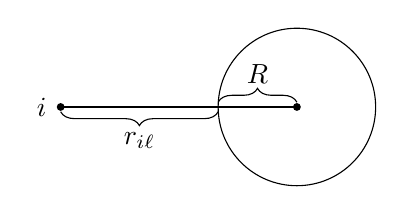
\begin{tikzpicture}

\draw(-3,0) -- (-1,0);
\node[circle,inner sep=1pt,fill=black,label=left:{$i$}] at (-3,0) {};
\draw[color=black] (0,0) circle [radius=1];
\draw(0,0) -- (-1,0);;
\node[circle,inner sep=1pt,fill=black,label=left:] at (0,0) {};

\draw [decorate,decoration={brace,amplitude=5pt,mirror,raise=0.4ex}]
  (0,0) -- (-1,0) node[midway,yshift=1.2em]{$R$};
  
\draw [decorate,decoration={brace,amplitude=5pt,mirror,raise=0.4ex}]
  (-3,0) -- (-1,0) node[midway,yshift=-1.2em]{$r_{i\ell}$};

\end{tikzpicture}
\end{center}
where \( r_{i \ell} \) represents the distance between robot and outside of obstacle and \( R \) is the radius of obstacle. 
Hence, 
\begin{align*}
    |r_{i\ell}(t)| = \sqrt{(x_i(t) - a_{\ell})^2 + (y_i(t) - b_{\ell})^2} - R
\end{align*}
and using a similar procedure to the previous section, we arrive at:
\begin{align*}
    G = \int_{0}^{1} \bigg(  \sum_{i=1}^{N}\sum_{\ell=1}^{M} \frac{1}{|r_{i\ell}(t)|^2}        \bigg) \ dt.
\end{align*}
So, in order to avoid hitting obstacles, we want to minimize the functional
\begin{align*}
    G(P) = G(P_1,...,P_N) =  \int_{0}^{1} \bigg( \sum_{i=1}^{N}\sum_{\ell=1}^{M} \frac{1}{|r_{i\ell}(t)|^2} \bigg) \ dt.
\end{align*}

